\documentclass[../../main.tex]{subfiles}

\begin{document}
\subsection{Arithmetic in GF(2)}
\subsubsection{Multiplication of Polynomials in GF(2)}
If we want to multiply $(x^5 + x^2 + 1)(x^3+1)$, we write the coefficients of the two polynomials in the form
\[
(x^5 + x^2 + 1)(x^3+1)\iff (5,\,2,\,0)(3,\,0)
\]
Find the set of sums across the two tuples, given by
\[
(8,\,5,\,5,\,2,\,3,\,0)
\]
Then retain only the ones that have an odd number of terms (here the two $5$ cancel out), and we get
\[
(8,\,3,\,2,\,0)\iff x^8 + x^3 + x^2 + x^0
\]
Let us try with another example with $(1+x)(x+x^2)$
\[
(1+x)(x+x^2)\iff (1,\,0)(1,\,2)
\]
The set of sums is $(2,\,3,\,1,\,2)$, and flipping the required coefficients we get
\[
(3,1)\implies (1+x)(x+x^2) = x^3 + x
\]
\subsubsection{Long Division of Polynomials in GF(2)}
Assume that $G(X) = (3,0) = x^3 + x^0$, and $D(X) = (3,1,0) = x^3 + x^1 + x^0$, if we wish to find $R(X)$ then we wish to find the remainder of $\frac{X^{3}D(X)}{G(X)}$\\
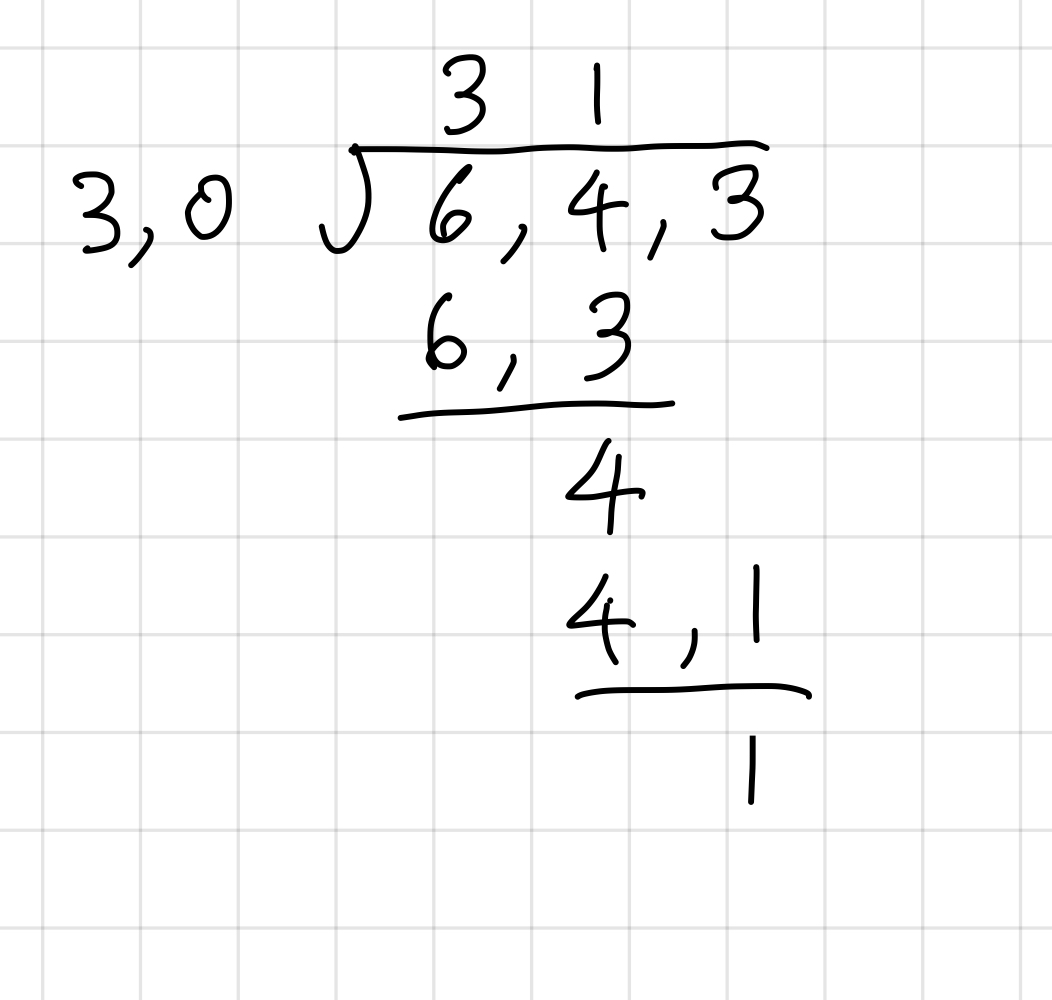
\includegraphics[width=.5\textwidth]{images/long_division_example_polynomial.jpeg}
\end{document}
